\chapter{Projetos Relacionados}

\section{Sistemas Existentes no Mercado}

\subsection{Sistemas Comerciais}
Atualmente, já percebe-se a existência de alguns sistemas comerciais de automação residencial - a maioria deles atuando de maneira mais forte do mercado Norte-Americano. Alguns dos sistemas mais populares nessa linha são o Amazon Echo e o Google Home.

O Amazon Echo consiste em um \texit{smart speaker} (alto falante inteligente) conectado ao assistente pessoal Alexa, também da empresa Amazon, que é capaz de entender comandos de voz. Inicialmente, funcionava como uma maneira de encomendar produtos por voz. Atualmente, além de funcionar como assistente pessoal, também é capaz de controlar diversos \texit{smart devices} da casa, funcionando como um \texit{hub} de automação residencial. Uma limitação deste produto é que funciona apenas com uma conexão \texit{wireless} de Internet, não sendo capaz de operar em nenhum nível sem a mesma.

Algumas características interessantes do Alexa são que desenvolvedores são capazes de adicionar novas \texit{skills} (habilidades) por meio de documentação da API que está pública e disponibilizada \texit{online}. Dessa forma, seu \texit{skillset} é passível de grande expansão e personalização. Além disso, o serviço de voz desse sistema, conhecido como Alexa Voice Service, pode ser utilizado por qualquer dispositivo que contenha microfone e alto falante e consiga conectar-se a ele pela Internet.

O Google Home é similar ao Amazon Echo em alguns aspectos, sendo também um \texit{smart speaker}, que surgiu como expansão do aplicativo para \texit{smartphones} Google Now (um assistente pessoal). Atualmente existe também como aplicativo para \texit{smartphones}. Não é possível o desenvolvimento de módulos e expansões ao Google Home por desenvolvedores desvinculados à Google, porém ela trabalha diretamente com outras marcas e produtos para o estabelecimento de parcerias que permitam integração com eles, de forma que o Google Home também consiga funcionar como \texit{hub} de automação residencial.

\subsection{Sistemas Open Source}
Também existem diversos projetos \texit{open source} sobre o tema, cujas documentações estão disponíveis publicamente online. Alguns desses projetos analisados para o desenvolvimento do nosso projeto Hedwig foram o OpenHAB e o Home Assistant.

O OpenHAB possui como objetivo principal o estabelecimento de uma plataforma em software de integração que seja capaz de solucionar o problema atual de que os diversos \texit{devices} de uma residência não são capazes de se comunicar devido à falta de uma linguagem comum com a qual eles possam estabelecer tal comunicação. Por ser independente de hardware específico, é extremamente flexível e personalizável, porém isso implica em certa complexidade para o usuário, no momento de sua instalação. Apresenta interface para o usuário em cliente web e aplicativos nativo para iOS e Android.

O Home Assistant é uma plataforma de automação residencial capaz de controlar e monitorar os diversos devices em uma casa, oferecendo uma plataforma web para o controle do sistema pelo usuário. O controlador local é implementado em Python, e recomenda-se instalá-lo em um Raspberry Pi. Possui diversas integrações já estabelecidas, com sistemas e serviços como o próprio Amazon Echo, Google Cast, IFTTT, Digital Ocean, entre outros, mas possibilita também a criação de novos componentes pelos próprios usuários. A personalização pelos usuários é feita por meio de um arquivo de configuração, no formato YAML.

Os dois projetos apresentam a dificuldade de que é necessário que o usuário possua conhecimentos técnicos para utilizá-los.

\section{Projeto HomeSky}

O Projeto HomeSky \cite{homeSky} é um Trabalho de Conclusão de Curso desenvolvido por alunos de Engenharia de Computação na Escola Politécnica da Universidade de São Paulo. Com o objetivo de fomentar iniciativas de desenvolvimento na área de casas inteligentes, o trabalho focou-se na criação do protocolo Rainfall, um protocolo em código aberto a nível de aplicação para ser usado na coordenação de uma rede de sensores. Isso permitiria aos desenvolvedores ter uma maior flexibilidade em seus projetos, visto que muitas das soluções existentes são proprietárias. Por fim, também foi realizada a implementação de um algoritmo de aprendizado de máquina capaz de controlar a iluminação.

\begin{figure}[H]
	\centering
	\caption{Camadas da arquitetura usada no Projeto HomeSky. As camadas em verde correspondem às bibliotecas desenvolvidas no trabalho.}
  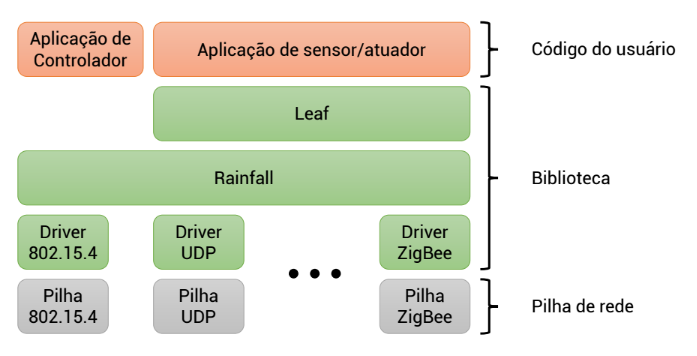
\includegraphics[width=0.8\textwidth]{arquiteturaHomeSky}
\label{fig:arquiteturaHomeSky}
\end{figure}

No desenvolvimento do protocolo Rainfall, foram consideradas algumas hipóteses simplificadoras a respeito da conectividade e da segurança. O protocolo não trata de forma especial a fase de conexão à rede, considerando que todos os nós já estão conectados a ela, e também considera que todos os protocolos adjacentes são confiáveis, deixando possíveis implementações de mecanismos de reconhecimento de entrega e retransmissão a cargo do desenvolvedor. Quanto à segurança, assume-se que a infraestrutura seja segura e que nenhum nó conectado à rede tenha comportamento mal intencionado, como por exemplo espionar mensagens destinadas a outros nós ou fingir ser o controlador.

O sistema Hedwig será uma evolução natural do Projeto HomeSky, buscando aperfeiçoar seu protocolo e arquitetura quanto à robustez e expandir a aplicação de aprendizado de máquina, além de viabilizar seu conceito, desenvolvendo soluções voltadas ao mercado brasileiro.
